% задание и сама лабораторная работа
% Для листинга кода:
\lstset{ %
	language=lisp,                 % выбор языка для подсветки (здесь это С++)
	basicstyle=\small\sffamily, % размер и начертание шрифта для подсветки кода
	numbers=left,               % где поставить нумерацию строк (слева\справа)
	numberstyle=\tiny,           % размер шрифта для номеров строк
	stepnumber=1,                   % размер шага между двумя номерами строк
	numbersep=5pt,                % как далеко отстоят номера строк от подсвечиваемого кода
	showspaces=false,            % показывать или нет пробелы специальными отступами
	showstringspaces=false,      % показывать или нет пробелы в строках
	showtabs=false,             % показывать или нет табуляцию в строках
	frame=single,              % рисовать рамку вокруг кода
	tabsize=2,                 % размер табуляции по умолчанию равен 2 пробелам
	captionpos=t,              % позиция заголовка вверху [t] или внизу [b] 
	breaklines=true,           % автоматически переносить строки (да\нет)
	breakatwhitespace=false, % переносить строки только если есть пробел
	escapeinside={\#*}{*)}   % если нужно добавить комментарии в коде
}
\newpage
\section*{Задание 1}
\addcontentsline{toc}{section}{\tocsecindent{Задание 1}}

\Large Проанализировать работу приведенных программ и объяснить результаты их работы.
\newline

\begin{lstlisting}[language=c,label=some-code1,caption=Программа 1]
#include <stdio.h>
#include <fcntl.h>

int main()
{
	// have kernel open connection to file alphabet.txt
	int fd = open("alphabet.txt",O_RDONLY);

	// create two a C I/O buffered streams using the above connection 
	FILE *fs1 = fdopen(fd,"r");
	char buff1[20];
	
	setvbuf(fs1,buff1,_IOFBF,20);

	FILE *fs2 = fdopen(fd,"r");
	char buff2[20];
	
	setvbuf(fs2,buff2,_IOFBF,20);

	// read a char & write it alternatingly from fs1 and fs2
	int flag1 = 1, flag2 = 2;
	
	while(flag1 == 1 || flag2 == 1)
	{
		char c;
		
		flag1 = fscanf(fs1,"%c",&c);
		
		if (flag1 == 1) 
		{
			fprintf(stdout,"%c",c);
		}
		
		flag2 = fscanf(fs2,"%c",&c);
		
		if (flag2 == 1) 
		{ 
			fprintf(stdout,"%c",c); 
		}
	}
	
	return 0;
}
\end{lstlisting} 

\textbf{Результаты работы:}

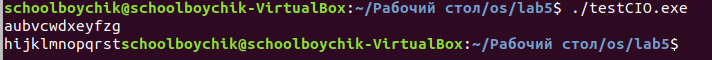
\includegraphics[scale=1]{img/Screenshot_1.png}

При первом вызове fscanf() буфер ввода fs1 заполняется до конца, то есть первыми 20 символами, после чего меняется значение текущей позиции. Поскольку fs1 и fs2 ссылаются на одну и ту же запись в системной таблице открытых файлов, то при следующем вызове fscanf() буфер ввода fs2 считает последние 6 символов из файла. Результатом вывода будет являться строка, в которой символы поочередно выводятся из первого и второго буферов (поскольку в одном буфере 20 символов, а в другом 6, "вперемешку" будут выведены только первые 12 символов).

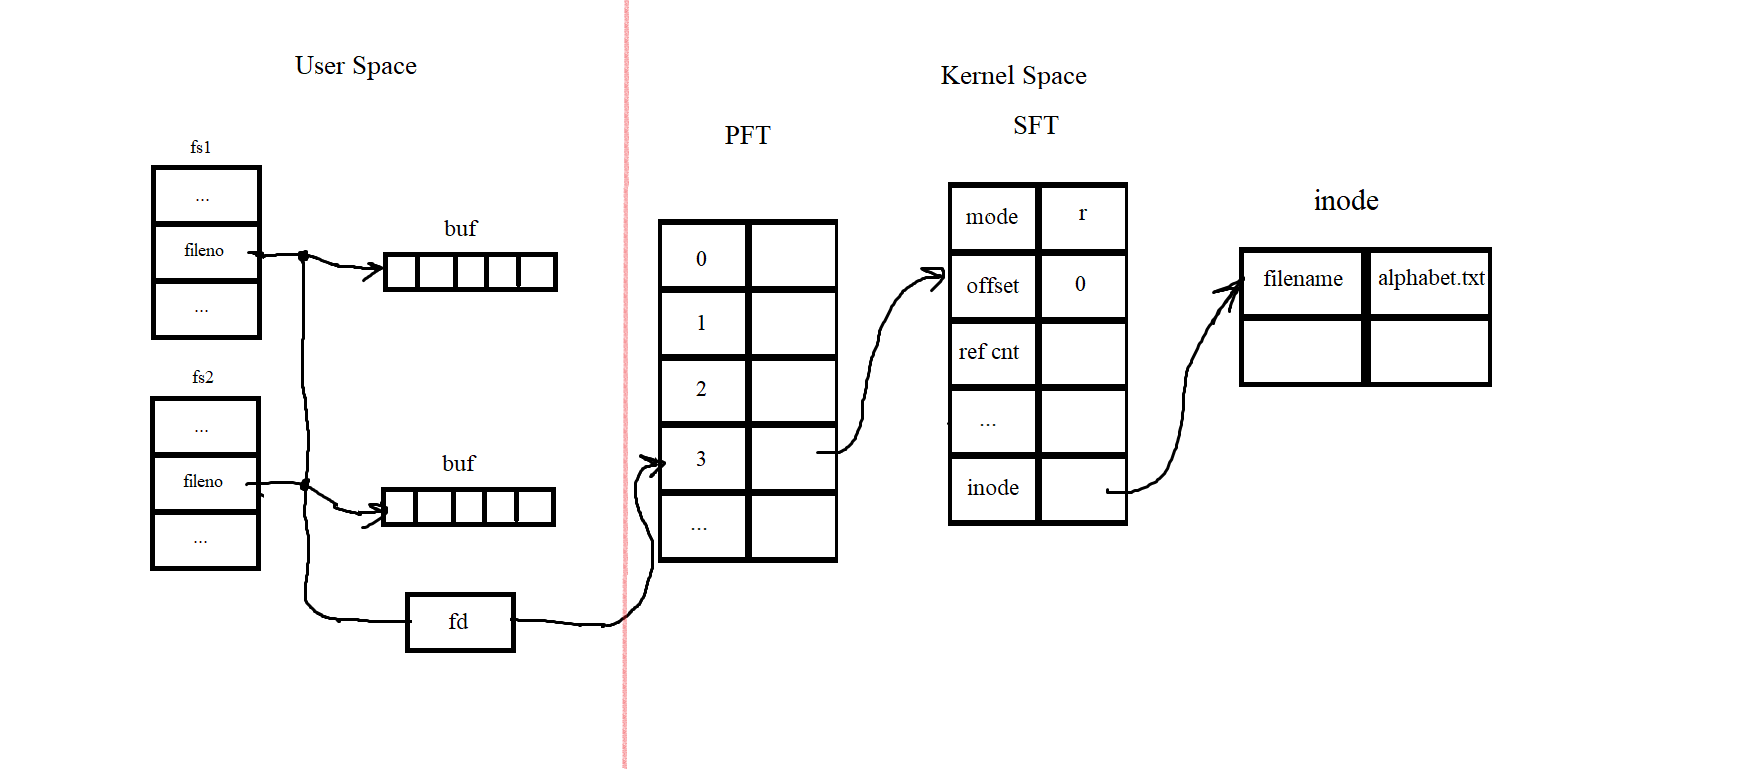
\includegraphics[scale=0.5]{img/1.png}
\newpage
\subsection*{Задание 1.2}
\addcontentsline{toc}{subsection}{\tocsecindent{Задание 1.2}}

\begin{lstlisting}[language=c,label=some-code2,caption=Программа 2]
#include <fcntl.h>
#include <stdio.h>

int main()
{
	char c;  
	  
	// have kernel open two connection to file alphabet.txt
	int fd1 = open("alphabet.txt",O_RDONLY);
	int fd2 = open("alphabet.txt",O_RDONLY);
	// read a char & write it alternatingly from connections fs1 & fd2

	while(read(fd1,&c,1) == 1 && read(fd2,&c,1) == 1)
	{
		write(1,&c,1);

		write(1,&c,1);
	}

	return 0;
}

\end{lstlisting} 

\textbf{Результаты работы:}

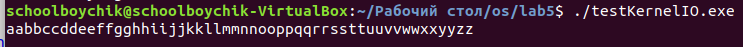
\includegraphics[scale=1]{img/Screenshot_2.png}

Системный вызов open() вызывается 2 раза, каждый раз создавая новый файловый дескриптор (а также новую запись в системной таблице открытых файлов). Поскольку файловые дескрипторы разные, у каждого своя текущая позиция, из-за чего в результате с помощью read() и write() получается строка с дублирующимися символами. 

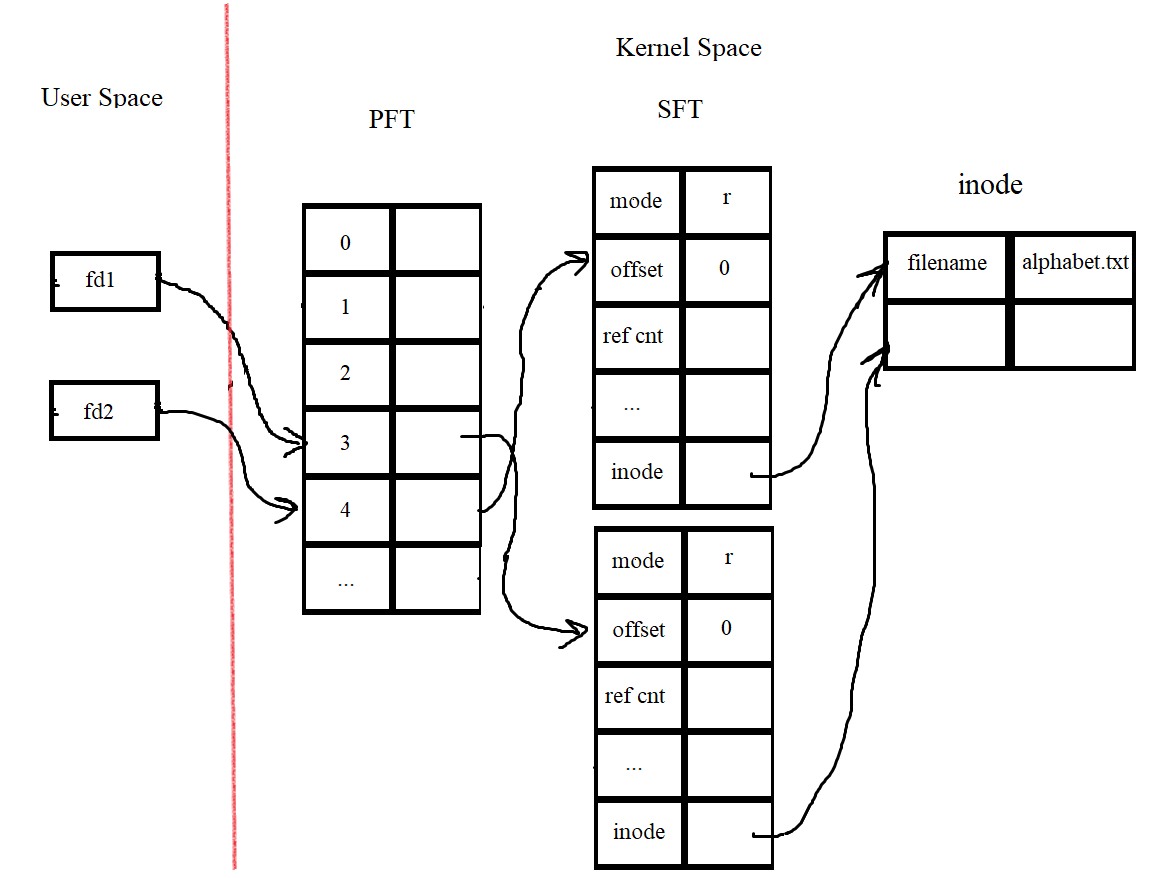
\includegraphics[scale=0.6]{img/2.png}
\newpage
\section*{Задание 2}
\addcontentsline{toc}{section}{\tocsecindent{Задание 2}}

\Large Написать программу, которая открывает один и тот же файл два раза с использованием библиотечной функции fopen(). Для этого объявляются два файловых дескриптора. В цикле записать в файл буквы латинского алфавита поочередно передавая функции fprintf() то первый дескриптор, то – второй.
Результат прокомментировать.\newline


\begin{lstlisting}[language=c,label=some-code3,caption=Программа 3]
#include <fcntl.h>
#include <stdio.h>

int main()
{
	char alph[26] = "abcdefghijklmnopqrstuvwxyz";

	FILE* f1 = fopen("p3.txt", "w");

	if (f1 == NULL)
	{
		return -1;
	}

	FILE* f2 = fopen("p3.txt", "w");

	if (f2 == NULL)
	{
		return -1;
	}

	for (int i = 0; i < 26; i++)
	{
		if (i % 2 == 0)
			fprintf(f1, "%c", alph[i]);

		if (i % 2 == 1)
			fprintf(f2, "%c", alph[i]);
	}

	fclose(f1);
	fclose(f2);

	return 0;
}

\end{lstlisting} 

\textbf{Результаты работы:}

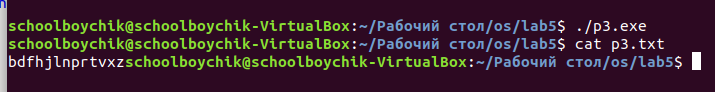
\includegraphics[scale=1]{img/Screenshot_3.png}

fprintf() обеспечивает буферизованный вывод, а значит запись файл происходит только при вызове функций fclose(), fflush() или заполнении буфера ввода. Функция fclose(f1) закроет файловый дескритор и очистит поток, на который указывает f1. После ее выполнения в файл будут записаны данные из первого потока. Затем fclose(f2) проделает то же самое с f2, но так как оба потока открыты на запись, данные, записанные с помощью первого потока перезапишутся данными из второго потока.

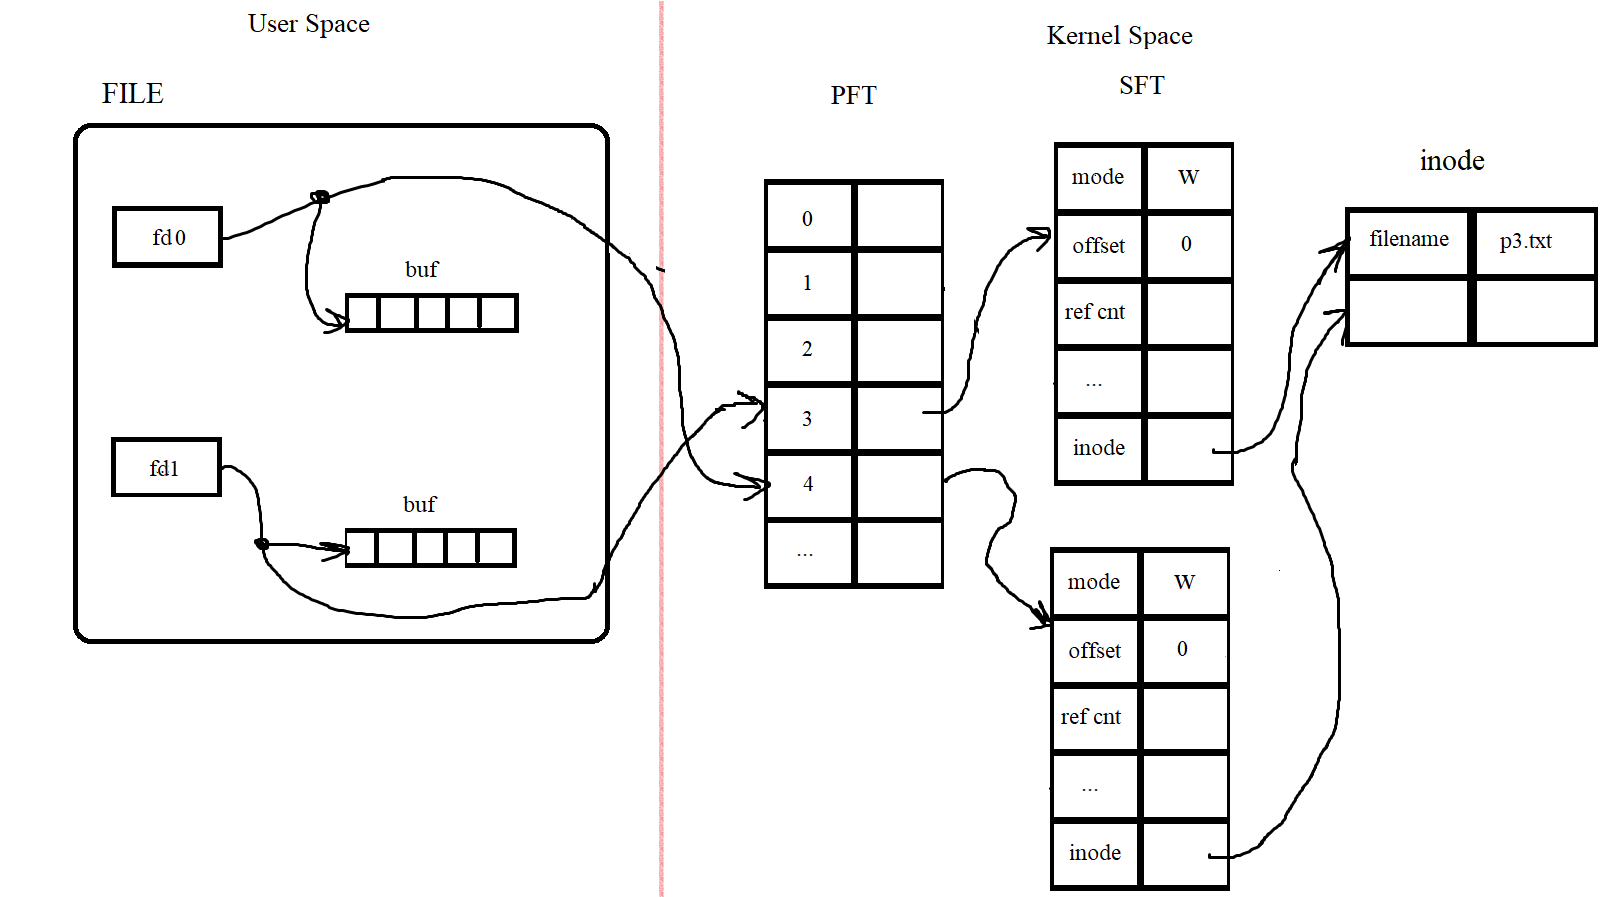
\includegraphics[scale=0.45]{img/3.png}
\newpage
\section*{Структура FILE}
\addcontentsline{toc}{section}{\tocsecindent{Структура FILE}}

Ниже приведена структура FILE.

\begin{lstlisting}[language=c,label=some-code4,caption=Структура FILE]
struct _IO_FILE {
int _flags;           /* High-order word is _IO_MAGIC; rest is flags. */
#define _IO_file_flags _flags

/* The following pointers correspond to the C++ streambuf protocol. */
/* Note:  Tk uses the _IO_read_ptr and _IO_read_end fields directly. */
char* _IO_read_ptr;   /* Current read pointer */
char* _IO_read_end;   /* End of get area. */
char* _IO_read_base;  /* Start of putback+get area. */
char* _IO_write_base; /* Start of put area. */
char* _IO_write_ptr;  /* Current put pointer. */
char* _IO_write_end;  /* End of put area. */
char* _IO_buf_base;   /* Start of reserve area. */
char* _IO_buf_end;    /* End of reserve area. */
/* The following fields are used to support backing up and undo. */
char *_IO_save_base; /* Pointer to start of non-current get area. */
char *_IO_backup_base;  /* Pointer to first valid character of backup area */
char *_IO_save_end; /* Pointer to end of non-current get area. */

struct _IO_marker *_markers;

struct _IO_FILE *_chain;

int _fileno;
#if 0
int _blksize;
#else
int _flags2;
#endif
_IO_off_t _old_offset; /* This used to be _offset but it's too small.  */

#define __HAVE_COLUMN /* temporary */
/* 1+column number of pbase(); 0 is unknown. */
unsigned short _cur_column;
signed char _vtable_offset;
char _shortbuf[1];

/*  char* _save_gptr;  char* _save_egptr; */

_IO_lock_t *_lock;
#ifdef _IO_USE_OLD_IO_FILE
};

struct _IO_FILE_complete {
struct _IO_FILE _file;
#endif
#if defined _G_IO_IO_FILE_VERSION && _G_IO_IO_FILE_VERSION == 0x20001
_IO_off64_t _offset;
# if defined _LIBC || defined _GLIBCPP_USE_WCHAR_T
/* Wide character stream stuff.  */
struct _IO_codecvt *_codecvt;
struct _IO_wide_data *_wide_data;
struct _IO_FILE *_freeres_list;
void *_freeres_buf;
size_t _freeres_size;
# else
void *__pad1;
void *__pad2;
void *__pad3;
void *__pad4;
size_t __pad5;
# endif
int _mode;
/* Make sure we don't get into trouble again.  */
char _unused2[15 * sizeof (int) - 4 * sizeof (void *) - sizeof (size_t)];
#endif
};
#ifndef __cplusplus
typedef struct _IO_FILE _IO_FILE;
#endif
typedef struct _IO_FILE FILE;

\end{lstlisting}
